\documentclass[11pt]{article}

% ---------- Packages (subset of Thesis-Draft/main.tex's preamble) ----------
\usepackage[margin=1in]{geometry}
\usepackage{amsmath,amssymb}
\usepackage{booktabs}
\usepackage{siunitx}
\usepackage[table]{xcolor}
\usepackage{tikz}
\usetikzlibrary{arrows.meta, positioning, fit, calc, backgrounds}
\usepackage[colorlinks=true, linkcolor=blue, citecolor=blue, urlcolor=blue]{hyperref}
\usepackage{enumitem}
\usepackage{float}
\usepackage{listings}
\setlength{\emergencystretch}{2em}

\lstset{basicstyle=\ttfamily\footnotesize, columns=fullflexible, breaklines=true,
        frame=single, rulecolor=\color{black!30}, keywordstyle=\bfseries,
        language=[Sharp]C}

\newcommand{\code}[1]{\texttt{#1}}

\title{Integrating Group Compression and Sidechain-Keyed Unmasking\\into a Unity VR Audio Pipeline}
\author{Implementation handoff --- demo\_engine $\rightarrow$ Unity 6000.4}
\date{}

\begin{document}
\maketitle

\begin{abstract}
This note specifies how the dynamic range processing developed in the demo
engine (sidechain-keyed unmasking, independent per-group compression, and an
output-bus WDRC stage) is carried into a Unity VR project in which
\code{AudioMixerGroup}s stand in for the source-separated stems. Because Unity
exposes no managed DSP hook inside a mixer group, the processing is split
between per-source taps and an end-of-block barrier on the
\code{AudioListener}. We show that this split is exactly equivalent to
processing each group bus, state its single block of latency and how to
remove it, define four listening conditions (``processing scenes''), and
report a parity test of the C\# reference implementation against the C++
engine on the Construction Scene stems.
\end{abstract}

% =====================================================================
\section{Processing scenes}
\label{sec:scenes}

Each scene is one listening condition, applied to $C=5$ classes $c$:
Dialogue, Music, Background Noise, Safety Alerts and Other.

\begin{table}[H]
\centering
\small
\caption{Processing scenes. Output WDRC is an independent toggle on any scene.}
\label{tab:scenes}
\begin{tabular}{@{}l p{2.6cm} p{3.4cm} p{4.6cm}@{}}
\toprule
\textbf{Scene} & \textbf{Group compression} & \textbf{Sidechain unmasking} & \textbf{Purpose} \\
\midrule
S0 Unprocessed & off & off & baseline \\
S1 Unmasked    & off & on (key $k$, Advanced) & make room for one priority group \\
S2 Compressed  & on, per group & off & raise quiet content in every group \\
S3 Combined    & on, per group & on (key $k$) & both, in series (Sec.~\ref{sec:combined}) \\
\bottomrule
\end{tabular}
\end{table}

In the C++ engine, Enhancement and Unmasking are mutually exclusive tabs, so
S3 is a new condition and its ordering is defined below.

% =====================================================================
\section{Architecture}
\label{sec:arch}

\subsection{Constraint}
Unity's managed API cannot insert DSP into an \code{AudioMixerGroup}. The
built-in mixer Compressor has no ratio or knee, and Duck Volume is full-band
only. The managed hooks available are \code{OnAudioFilterRead} on an
\code{AudioSource} (per source, pre-mixer) and on the \code{AudioListener}
(once per DSP block, after all sources and groups are mixed).

\subsection{Taps and barrier}
Let source $i$ belong to class $c(i)$ and let $\mathcal{S}_c$ be the set of
sources routed to the group(s) mapped to class $c$. The group signal is
\begin{equation}
  x_c(n) = \sum_{i \in \mathcal{S}_c} x_i(n).
  \label{eq:groupsum}
\end{equation}
In each DSP block of $N$ frames:
\begin{enumerate}[nosep]
  \item every source's \code{StemTap} adds its mono signal
        $\tfrac{1}{2}(x_i^L + x_i^R)$ (and, for multiband compression, its six
        band signals) into its class accumulator, which yields
        \eqref{eq:groupsum};
  \item the \code{UnmaskingListener} callback, which Unity runs after every
        source has been pulled, acts as a barrier: all group detectors run
        sample by sample over the accumulated block and write per-sample gain
        curves;
  \item each tap applies its class's gain curves to its own samples.
\end{enumerate}

\subsection{Equivalence to group-bus processing}
Every gain is a per-sample scalar $g_c(n)$ (or a per-sample, per-band scalar
$g_{c,b}(n)$), and the band splits $H_b$ are linear and time-invariant, so
\begin{equation}
  \sum_{i \in \mathcal{S}_c} \sum_b g_{c,b}(n)\,(H_b * x_i)(n)
  \;=\; \sum_b g_{c,b}(n)\,\Bigl(H_b * \sum_{i\in\mathcal{S}_c} x_i\Bigr)(n).
  \label{eq:equiv}
\end{equation}
Compressing every member of a group with the group's gain is therefore
identical to compressing the group bus. This is the same argument as the
engine's \code{SummedBus} ducking mode. Equation~\eqref{eq:equiv} is
confirmed numerically in Sec.~\ref{sec:verify}.

\begin{figure}[H]
\centering
\resizebox{\linewidth}{!}{%
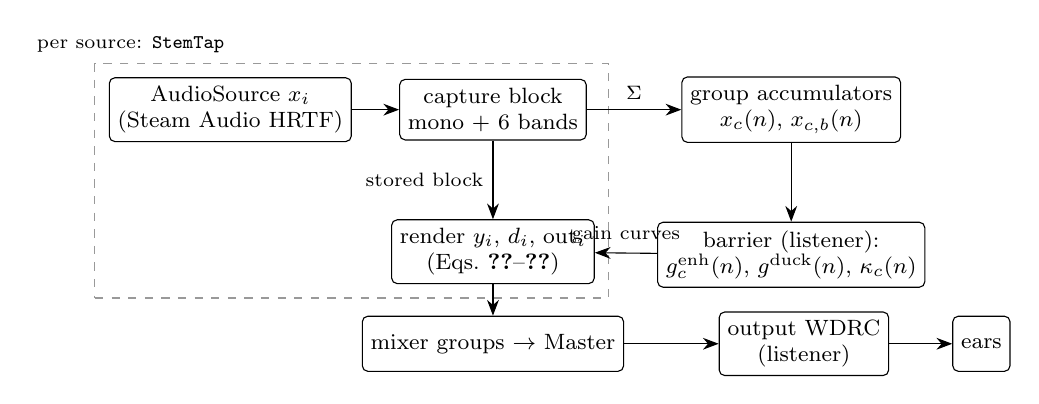
\begin{tikzpicture}[
  box/.style={draw, rounded corners=2pt, align=center, font=\footnotesize, minimum height=7mm, inner sep=3pt},
  arr/.style={-{Stealth[length=2mm]}},
  node distance=4mm and 6mm]
  % per-source column
  \node[box] (src) {AudioSource $x_i$\\(Steam Audio HRTF)};
  \node[box, right=of src] (cap) {capture block\\mono + 6 bands};
  \node[box, right=12mm of cap] (acc) {group accumulators\\$x_c(n)$, $x_{c,b}(n)$};
  \node[box, below=10mm of acc] (det) {barrier (listener):\\$g^{\mathrm{enh}}_{c}(n)$, $g^{\mathrm{duck}}(n)$, $\kappa_c(n)$};
  \node[box, below=10mm of cap] (ren) {render $y_i$, $d_i$, $\mathrm{out}_i$\\(Eqs.~\ref{eq:enh}--\ref{eq:out})};
  \node[box, below=of ren] (mix) {mixer groups $\rightarrow$ Master};
  \node[box, right=12mm of mix] (wdrc) {output WDRC\\(listener)};
  \node[box, right=8mm of wdrc] (ear) {ears};
  \draw[arr] (src) -- (cap);
  \draw[arr] (cap) -- node[above, font=\scriptsize]{$\Sigma$} (acc);
  \draw[arr] (acc) -- (det);
  \draw[arr] (det) -- node[above, font=\scriptsize]{gain curves} (ren);
  \draw[arr] (cap) -- node[left, font=\scriptsize]{stored block} (ren);
  \draw[arr] (ren) -- (mix);
  \draw[arr] (mix) -- (wdrc);
  \draw[arr] (wdrc) -- (ear);
  \begin{scope}[on background layer]
    \node[draw, dashed, black!40, fit=(src)(cap)(ren), inner sep=5pt, label={[font=\scriptsize]above left:per source: \code{StemTap}}] {};
  \end{scope}
\end{tikzpicture}}
\caption{Per-source taps feed group accumulators; the listener-callback
barrier computes group gains that the taps apply.}
\label{fig:flow}
\end{figure}

% =====================================================================
\section{Signal flow equations}
\label{sec:equations}

The detector and gain law are the engine's Eq.~1 and Eq.~2, unchanged. The
envelope is
\begin{equation}
  L(n) = \alpha\,L(n-1) + (1-\alpha)\,20\log_{10}\!\bigl(|u(n)|+\epsilon\bigr),
  \qquad
  \alpha = \begin{cases} e^{-1/(\tau_A f_s)} & \text{rising}\\ e^{-1/(\tau_R f_s)} & \text{falling}\end{cases}
\end{equation}
and the soft-knee gain $G(L; T, R, W)$, in dB, is
\begin{equation}
  G = \begin{cases}
   0 & L < T - W/2\\
   \left(\tfrac{1}{R}-1\right)\dfrac{(L-T+W/2)^2}{2W} & |L-T|\le W/2\\
   \left(\tfrac{1}{R}-1\right)(L-T) & L > T + W/2.
  \end{cases}
\end{equation}

\paragraph{Group compression (Enhancement).}
Each class $c$ has its own threshold $T_c$, ratio $R_c$, knee $W_c$,
attack $\tau_{A,c}$, release $\tau_{R,c}$ and makeup gain $m_c$. In single-band mode the detector reads the group mono
sum $u=x_c$, and in multiband mode it reads each of the six band sums
$u=x_{c,b}$ (crossovers at 100, 299, 894, 2675, \SI{8000}{\hertz}) with
$+\SI{10}{\decibel}$ level compensation. With $\beta(n)$ the 25\,ms on/off
crossfade, the output for source $i$ in class $c$ is
\begin{align}
  \text{single-band:}\quad y_i(n) &= \bigl[(1-\beta) + \beta\, m_c\, g_c(n)\bigr]\, x_i(n), \label{eq:enh}\\
  \text{multiband:}\quad y_i(n) &= (1-\beta)\,x_i(n) + \beta\, m_c \textstyle\sum_b g_{c,b}(n)\,(H_b * x_i)(n). \nonumber
\end{align}

\paragraph{Sidechain unmasking.}
The key detector reads the key group's mono sum $x_k$, gated by the
key-detector tap choice (Sec.~\ref{sec:combined}). The duck gain is clamped
by the maximum reduction $D_{\max}$ and faded by the unmask on/off ramp
$u(n)$:
\begin{equation}
  g^{\mathrm{duck}}(n) = 1 + u(n)\Bigl(\max\bigl\{10^{G/20},\,10^{-D_{\max}/20}\bigr\} - 1\Bigr).
\end{equation}
Basic mode ducks full-band. Advanced mode ducks only the key class's range
$[f_\ell(k), f_h(k)]$ via two LR4 splits per channel:
\begin{equation}
  d_i(n) = \begin{cases}
   g^{\mathrm{duck}}(n)\,y_i(n) & \text{Basic}\\
   y_i^{<f_\ell}(n) + y_i^{>f_h}(n) + g^{\mathrm{duck}}(n)\,y_i^{[f_\ell,f_h]}(n) & \text{Advanced.}
  \end{cases}
\end{equation}

\paragraph{Key crossfade and output.}
With $\kappa_c(n)\in[0,1]$ ramping to 1 for the key class (30\,ms) and
static key gain $s$ (the engine's \code{safetyGainDb}):
\begin{equation}
  \mathrm{out}_i(n) = \kappa_{c(i)}(n)\, s\, y_i(n) + \bigl(1-\kappa_{c(i)}(n)\bigr)\, d_i(n).
  \label{eq:out}
\end{equation}
The outputs then pass through Steam Audio and the mixer, and the 6-band
output WDRC runs on the final mix in the listener callback.

\subsection{Combined scene}
\label{sec:combined}
Group compression precedes ducking (Eqs.~\ref{eq:enh}--\ref{eq:out}). The
key-detector input is a research choice:
\begin{itemize}[nosep]
  \item \textbf{Pre-enhancement} (default): $u = x_k$. Thresholds calibrated
        in the thesis sweeps on raw stems remain meaningful.
  \item \textbf{Post-enhancement}: $u$ is the key group after its own
        compression and makeup, which is what the listener hears. Positive
        makeup on the key deepens the duck.
\end{itemize}
Both are computable at the barrier from the accumulated sums, because the
group gains are already known there.

% =====================================================================
\section{Latency}
\label{sec:latency}

The group gain for block $j$ exists only at the end of block $j$. With
\emph{Align} on, each tap outputs its previous block, so gain and audio are
sample-aligned at the cost of $N/f_s$ extra latency. With Align off, the
current block receives the previous block's gain, so the detector is one block
late. Table~\ref{tab:lag} measures the Align-off error against the
sample-accurate C++ engine (Advanced, Dialogue key, Construction Scene).

\begin{table}[H]
\centering
\small
\caption{Detector-lag error with Align off. The target project currently uses
$N=1024$. The recommendation is $N=256$ with Align on (\SI{5.3}{\milli\second} added latency, exact).}
\label{tab:lag}
\begin{tabular}{@{}S[table-format=4.0] S[table-format=2.1] S[table-format=-2.1] S[table-format=-2.1]@{}}
\toprule
{$N$ (frames)} & {Lag (\si{\milli\second})} & {Peak error (dBFS)} & {RMS error (dBFS)} \\
\midrule
256  & 5.3  & -27.4 & -69.7 \\
512  & 10.7 & -27.4 & -65.0 \\
1024 & 21.3 & -25.2 & -59.5 \\
\bottomrule
\end{tabular}
\end{table}

% =====================================================================
\section{Mapping onto the target project}
\label{sec:mapping}

\begin{table}[H]
\centering
\small
\caption{Mixer group $\rightarrow$ class mapping for \code{Main Mixer.mixer}
(Maybe VR). Map leaf groups that sources route to directly.}
\begin{tabular}{@{}lll@{}}
\toprule
\textbf{Mixer group} & \textbf{Class} & \textbf{Notes} \\
\midrule
Dialogue & Dialogue & \code{TestZone} dialogue sources \\
Music & Music & \\
Background Noise, OutdoorSurrounds & Background Noise & two groups, one class \\
Randomized FX & Safety Alerts (or Other) & embedded detection cues \\
REVERB & (unmapped) & shared return, unprocessed \\
\bottomrule
\end{tabular}
\end{table}

\paragraph{Spatialization.}
With \code{spatializePostEffects = false} (the Unity default), the tap
follows the Steam Audio spatializer, so the detector measures the binaural,
distance-attenuated signal at the ears. This is the closer analog to a hearing
aid's separated streams, and it is the recommended choice. With
\code{true}, the detector measures the dry source. The gain is a slowly
varying scalar, so its placement relative to the linear HRTF matters only
within the attack time.

\paragraph{Scenes.}
Each condition is a \code{ProcessingScene} asset holding all parameters and
an optional \code{AudioMixerSnapshot} for static fader balance. Use the
snapshot to loudness-match conditions. The reference renders measured RMS of
$-29.4$, $-30.4$, $-30.2$ and $-30.9$\,dBFS for S0--S3, so unmatched
conditions are confounded by level. Scenes are applied between trials;
\code{TrialRecord} should log the scene identifier and the per-trial telemetry
(engaged fraction, mean and minimum duck gain, minimum group-compression gain).

\paragraph{Calibration.}
Thresholds are absolute dBFS at the detector, and VR playback levels differ
from the stem levels used in the sweeps. The sweeps showed threshold dominates
($r=-0.929$ with margin gain), so calibrate in-scene by the duck's
\emph{engaged fraction}: about \SI{69}{\percent} (Aggressive),
\SI{30}{\percent} (Balanced), or \SI{2}{\percent} (Conservative). Keep each
tier's ratio, knee and time constants.

% =====================================================================
\section{Verification of the reference implementation}
\label{sec:verify}

The C\# port (\code{unity/Runtime/}) keeps its DSP core free of UnityEngine.
It was driven exactly as Unity's audio thread drives it (all source filters,
then the listener filter, in 1024-frame blocks) on \SI{30}{\second} of the
Construction Scene stems, and compared with the C++ \code{Engine}.

\begin{table}[H]
\centering
\small
\caption{Parity of the Unity C\# port (Align on) against the C++ engine.
Maximum absolute sample difference.}
\label{tab:parity}
\begin{tabular}{@{}lS[table-format=-3.1]l@{}}
\toprule
\textbf{Scenario} & {\textbf{Max diff (dBFS)}} & \textbf{Note} \\
\midrule
Unprocessed                    & {exact} & \\
Basic, Dialogue key            & -150.5 & \\
Advanced, Dialogue key         & -150.5 & \\
Advanced, Safety key, $+3$\,dB key gain & -144.5 & \\
Enhancement, single-band       & -144.5 & \\
Enhancement, multiband         & -113.5 & C++ internal 25\,ms startup fade residue \\
Advanced + output WDRC         & -142.6 & after 0.5\,s startup \\
\midrule
Group equivalence, Eq.~\eqref{eq:equiv} (all scenes) & -147.0 & worst case \\
S3 with Enhancement off $\equiv$ S1 & {exact} & \\
S3 with Unmask off $\equiv$ S2 & {exact} & \\
\bottomrule
\end{tabular}
\end{table}

The Unity components compile against Unity 6000.4.10f1's managed assemblies
but have not yet been run in the editor.

% =====================================================================
\section{Not ported and alternatives}
\begin{itemize}[nosep]
  \item \textbf{Resonance mode} (STFT, $2048$-point, \SI{43}{\milli\second}
        latency) would need a per-source STFT with the mask built at the
        barrier from the key group's spectrum. It is CPU-heavy in managed
        code on standalone headsets.
  \item \textbf{Per-channel Advanced thresholds} are not ported (a small extension).
  \item \textbf{Reverb returns} and other unmapped groups are unprocessed.
  \item \textbf{Native alternative:} a Unity Native Audio Plugin wrapping the
        existing C++ headers as mixer effects, with the key routed by
        Send $\rightarrow$ sidechain target. It gives group-level DSP with no
        block lag, at the cost of per-platform native builds.
\end{itemize}

\end{document}
